\documentclass[english,notitlepage,reprint,nofootinbib]{revtex4-1}  % defines the basic parameters of the document
% For preview: skriv i terminal: latexmk -pdf -pvc filnavn
% If you want a single-column, remove "reprint"
% Allows special characters (including æøå)
\usepackage[utf8]{inputenc}
% \usepackage[english]{babel}

%% Note that you may need to download some of these packages manually, it depends on your setup.
%% I recommend downloading TeXMaker, because it includes a large library of the most common packages.

\usepackage{physics,amssymb}  % mathematical symbols (physics imports amsmath)
\include{amsmath}
\usepackage{graphicx}         % include graphics such as plots
\usepackage{xcolor}           % set colors
\usepackage{hyperref}         % automagic cross-referencing
\usepackage{listings}         % display code
%\usepackage{subfigure}        % imports a lot of cool and useful figure commands
\usepackage{float}
%\usepackage[section]{placeins}
\usepackage{algorithm}
\usepackage[noend]{algpseudocode}
\usepackage{subfigure}
\usepackage{tikz}
\usepackage{mathrsfs}
\bibliographystyle{apsrev4-1}
\usetikzlibrary{quantikz}
% defines the color of hyperref objects
% Blending two colors:  blue!80!black  =  80% blue and 20% black
\hypersetup{ % this is just my personal choice, feel free to change things
    colorlinks,
    linkcolor={red!50!black},
    citecolor={blue!50!black},
    urlcolor={blue!80!black}}
% ===========================================


\begin{document}

\title{A study of phase transition in the 2D Ising model\\using Markov Chain Monte Carlo simulation}  % self-explanatory
\author{Alessio Canclini, Filip von der Lippe} % self-explanatory
\date{\today}                             % self-explanatory
\noaffiliation                            % ignore this, but keep it.

%This is how we create an abstract section.
\begin{abstract}
    This article looks at phase transition in the widely studied Ising model. We attempt a numerical approximation of the critical temperature at which an infinite lattice Ising model undergoes phase change using a Markov Chain Monte Carlo approach (MCMC).
    The MCMC method is first
\end{abstract}
\maketitle
\raggedbottom


% ===========================================
\section{Introduction}\label{sec:intro}
This article will explore temperature-dependent behavior in ferromagnetism using the two-dimensional \textbf{Ising model}. The main purpose of our simulations is to determine a numerical estimation of the \textbf{critical temperature} at which the system transitions from a magnetized to a non-magnetized phase. This is also called the Curie temperature. Past this point the magnetic spins are no longer aligned, causing the given ferromagnetic material to lose its magnetization.

With the Ising model we can easily model a magnetic materials' response to thermal energy. Magnet spins in the model have two states, either up or down. These can be flipped by energy input and each individual spin influences the total state of the system.

The Ising model is a widely studied model in statistical physics. Work on the model has shown to be useful for the analysis of several complex systems. Some examples are gasses sticking to solid surfaces or hemoglobin molecules that absorb oxygen. Additionally, when it comes to studies of phase transition, theoretical approaches such as mean field models can actually predict wrong behavior, further motivating the use of the Ising model.\cite{compendium}

We will simulate the Ising model using a Markov Chain Monte Carlo (MCMC) approach. After testing our numerical method we will finally try to approximate the critical temperature for an infinite $(L=\infty)$ 2D Isisng model. The analytical solution to this problem was found by Lars Onsager in 1944 \cite{project}. Thus, our goal is not to necessarily find this temperature, but rather analyze how well our chosen MCMC approach can approximate such a complex problem.

To allow for reasonable runtimes for the larger computations our MCMC code is parallelized using OpenMP.

Section \ref{sec:methods} will cover the theoretical background of the Ising model and MCMC method as well as some analytical solutions for code testing. More comprehensive derivations of the analytical values can be found in appendix \ref{appendix:analytic} and \ref{appendix:delta_E}.

In section \ref{sec:results} we present results from our Ising model simulations. These cover comparison betwween analytic and numerical results, an analysis of burn-in time for a larger lattice size of $L = 20$ and finally an investigation of phase transitions.

A detailed discussion of the results and methods is then presented in section \ref{sec:discussion} followed by a summary and concluding thoughts in section \ref{sec:conclusion}.

% ===========================================
\section{Methods}\label{sec:methods}
A GitHub repository containing code and more information on how to reproduce the results of this report can be found following this link:
\url{https://github.com/Fslippe/FYS4150/tree/main/project4}


The square 2D lattices for our Ising model will have a length of $L$ containing $N$ spins with the relation $N = L^2$. Each spin $s_i$ will have two possible states of
\begin{equation*}
    s_i = -1 \text{ or } s_i = +1.
\end{equation*}
The total spin state or \textbf{spin configuration} of a lattice will be represented as $\textbf{s} = (s_1, s_2, ..., s_N)$. In its simplest form the total energy of the system is expressed as
\begin{equation*}
    E(\textbf{s}) = - J \sum^N_{\langle kl \rangle} s_k s_l - \mathscr{B} \sum^N_{k} s_k.
\end{equation*}
Here $\mathscr{B}$ is an external magnetic field. Since we will be looking at the Ising model without an external magnetic field the equation will be simplified to
\begin{equation}
    E(\textbf{s}) = - J \sum^N_{\langle kl \rangle} s_k s_l,
\end{equation}
where $\langle kl \rangle$ denotes the sum going over all \textit{neighboring pairs} of spins avoiding double-counting. $J$ is the \textbf{coupling constant} simply setting the energy associated with spin interactions. \textit{Periodic boundary conditions} will be implemented allowing all spins to have four neighbors.
\begin{equation}
    M(\textbf{s}) = \sum^N_i s_i
\end{equation}
is the magnetization of the entire system expressed as a sum over all spins. The energy per spin is
\begin{equation}
    \epsilon(\textbf{s}) = \frac{E(\textbf{s})}{N} \label{eq:mean_E}
\end{equation}
and the magnetization per spin is given by
\begin{equation}
    m(\textbf{s}) = \frac{M(\textbf{s})}{N}. \label{eq:mean_M}
\end{equation}
These values will be used to compare and analyze results.
\begin{equation}
    \beta = \frac{1}{k_B T}
\end{equation}
describes the ``inverse temperature'' with the systems' temperature $T$ and the Boltzmann constant $k_B$.
\begin{equation}
    Z = \sum_{\text{all possible \textbf{s}}} e^{- \beta E(\textbf{s})}
\end{equation}
represents the partition function. This, the `inverse temperature'' and the total energy of the system appear in the \textit{Boltzmann distribution},
\begin{equation}
    p(\textbf{s};T) = \frac{1}{Z} e^{-\beta E(\textbf{s})}.\label{eq:prob_dist}
\end{equation}
This will be the probability distribution used for random sampling in our Monte Carlo approach.


For comparison with early numerical implementations we will first consider an analytical solution. The following table \ref*{tab:analytic} summarizes all sixteen possible \textbf{spin configurations} of a $2 \cross 2$ lattice with \textit{periodic boundary conditions}.

% Please add the following required packages to your document preamble:
% \usepackage[table,xcdraw]{xcolor}
% If you use beamer only pass "xcolor=table" option, i.e. \documentclass[xcolor=table]{beamer}
\begin{table}[H]
    \centering
    \caption{Analytic values for the sixteen \textbf{spin configurations} of the $2 \cross 2$ Ising model lattice.}
    \begin{tabular}{|l|l|l|l|}
        \hline
        \begin{tabular}[c]{@{}l@{}}Nr. of spins \\ in state +1\end{tabular} & Degeneracy & \begin{tabular}[c]{@{}l@{}}Total \\ energy\end{tabular} & \begin{tabular}[c]{@{}l@{}}Total \\ magnetization\end{tabular} \\ \hline
        \hline
        0                          & 1          & -8J                        & -4                         \\    \hline
        1                          & 4          & 0                          & -2                         \\    \hline
        2                          & 4          & 0                          & 0                          \\    \hline
        2                          & 2          & 8J                         & 0                          \\    \hline
        3                          & 4          & 0                          & 2                          \\    \hline
        4                          & 1          & -8J                        & 4                          \\    \hline
    \end{tabular} \label{tab:analytic}
\end{table}
Based on the values in table \ref{tab:analytic} we derive the specific analytical expressions for the $2 \cross 2$ lattice case. The calculations of these analytic solutions can be found in appendix \ref{appendix:analytic} and are used to test early versions of the code.

We will study properties of the system at equilibrium for different lattice sizes as a function of temperature $T$. The analysis will focus on four main properties. The mean energy (eq. \ref{eq:mean_E}), mean magnetization (eq. \ref{eq:mean_M}), specific heat capacity normalized to number of spins
\begin{equation}
    C_V = \frac{1}{N} \frac{1}{k_B T^2} \left( \langle E^2 \rangle - \langle E \rangle^2 \right),
\end{equation}
and the susceptibility normalized to number of spins
\begin{equation}
    \chi = \frac{1}{N} \frac{1}{k_B T} \left( \langle M^2 \rangle - \langle |M| \rangle^2 \right).
\end{equation}
Analytical solutions to these can also be found in appendix \ref{appendix:analytic}.


\subsection*{Markov chain Monte Carlo and the metropolis algorithm}
We start with an initial energy computed from the random or ordered initial configuration of spins. We randomly flip one spin and calculate a temporary energy which we use to calculate $\Delta E$ which can take 5 different values. This gives us the possibility to use the returned value as an index which matches with the pre-calculated $w= e^{-\beta \Delta E}$. We then check if $w$ is larger or equal some random number in the interval [0,1] and if so, we accept the new flipped configuration. If not we keep the old configuration which allows us to move towards the energy minimum for the given temperature. We update the total energy and magnetization of the lattice if the configuration is changed. We repeat this $N$ times before we use the last calculated $M$ and $E$ to add to cumulative sums of $E$, $E^2$, $M$, $M^2$ and $|M|$. This is one Monte Carlo cycle and is repeated for a chosen number of cycles before an average of the cumulative sums is taken. In total can the metropolis algorithm together with the Monte Carlo sampling be viewed as a Markov Chain from how the probability to transition to a new state only is dependent on the current state spin configuration and following energy and magnetization.

A flow chart of the Metropolis algorithm can be found in appendix \ref{appendix:metro}.

\subsection*{Critical phenomena}
The final goal for the MCMC simulations will be to approximate the critical temperature for an \textit{infinite} $(L=\infty)$ 2D Ising model. As mentioned in section \ref{sec:intro}, the analytical solution for this was found by Lars Onsager. His result is
\begin{equation*}
    T_{c \text{ analytic}}(L=\infty) = \frac{2}{\ln(1+\sqrt{2})}J/k_B \approx 2.269 J/k_B.
\end{equation*}
For our approximation we will use the scaling relation
\begin{equation}
    T_c(L) -T_c(L=\infty) = aL^{-1}. \label{eq:scaling_rel}
\end{equation}
Here $a$ is constant. Theoretical background for this scaling relation can be found in appendix \ref{appendix:critical}. Eq. \ref{eq:scaling_rel} can be rearranged to the linear function
\begin{equation}
    T_c(L) = aL^{-1} + T_c(L=\infty). \label{eq:scaling_linear}
\end{equation}
This relation will be approximated by performing linear regression using the scipy package in python. The data set used will be $T_C$ values for different lattice sizes $L$ from plots of $C_V$ and $\chi$. In other words, the temperature at which $C_V$ and $\chi$ reach their peak value for different lattice sizes. The linear regression resulting in
\begin{equation}
    y = ax + b
\end{equation}
will thus supply a value for $a$ and the interception point $b$ which in this case is $T_c(L=\infty)$.

\subsection*{Optimization and parallelization}
%\subsection*{Periodic boundary conditions}
The Ising model simulations we will be implemented using periodic boundary conditions. This way, all spins will have four neighbors as seen in table \ref{fig:neighbors}, also at the boundaries of the lattice.
\begin{figure}[H]
    \centering
    \begin{tabular}{llll}
                   & $\uparrow$ &            \\
        $\uparrow$ & $\uparrow$ & $\uparrow$ \\
                   & $\uparrow$ &
    \end{tabular}\label{fig:neighbors}
    \caption{An example of a spin and its four neighbors. Here all five spins are in an up state (+1).}
\end{figure}
Periodic boundaries could be implemented using if-tests, but if-tests within loops can be slow. To make the code slightly more efficient we have chosen to write a \texttt{periodic} function using the modulo operator.

The Monte Carlo method will repeatedly require the Boltzmann factor $e^{-\beta \Delta E}$. The energy shift induced by flipping a single spin
\begin{equation}
    \Delta E = E_{\text{after}} - E_{\text{before}}
\end{equation}
can only take five possible values in a 2D-lattice of arbitrary size($L > 2$) This is shown in appendix \ref{appendix:delta_E}. These values are
\begin{equation}
    \Delta E = 8J, 4J, 0, -4J, -8J.
\end{equation}
To reduce computational cost we will avoid repeatedly calling the exponential function. This is done by pre-computing the five possible Boltzmann factors in an array.
Furthermore, the code is written such that it can be run parallelized. This allows us to run it on several threads using OpneMP to reduce runtimes.

% ===========================================
\section{Results}\label{sec:results}
To check the numerical implementation we compare analytical and numerical results for a $2\times2$ lattice case for $T=[0.5,4.0]J/k_B$ in the following figures.

\begin{figure}[H]
    \centering
    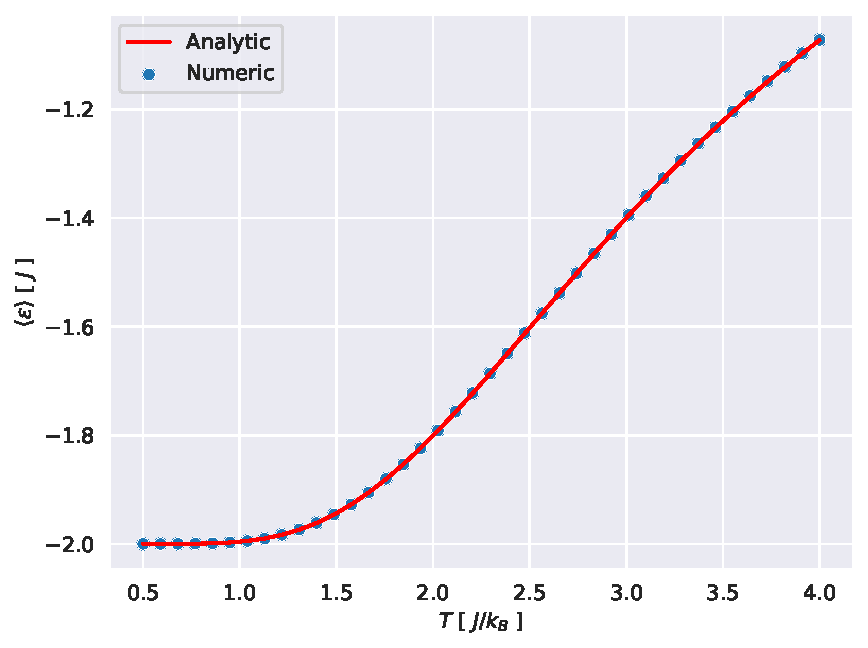
\includegraphics[width=.5\textwidth]{../figures/numeric_analytic_e_T.pdf}
    \caption{Comparison of the red analytic and blue numeric results in a $2\times2$ lattice case. Here one sees the expectation value for the energy per spin $\epsilon$ plotted against different temperatures $T$. Numerical results shown are for $10^6$ MC cycles.}
    \label{fig:numeric_analytic_e_T}
\end{figure}

\begin{figure}[H]
    \centering
    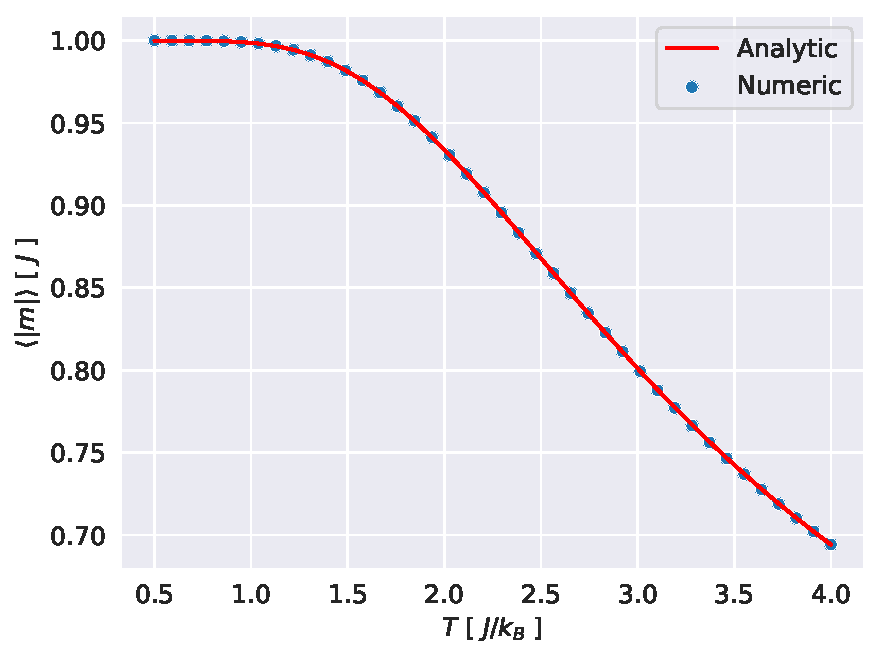
\includegraphics[width=.5\textwidth]{../figures/numeric_analytic_m_T.pdf}
    \caption{Comparison of the red analytic and blue numeric results in a $2\times2$ lattice case. Here one sees the expectation value for the magnetization per spin $m$ plotted against different temperatures $T$. Numerical results shown are for $10^6$ MC cycles.}
    \label{fig:numeric_analytic_m_T}
\end{figure}

\begin{figure}[H]
    \centering
    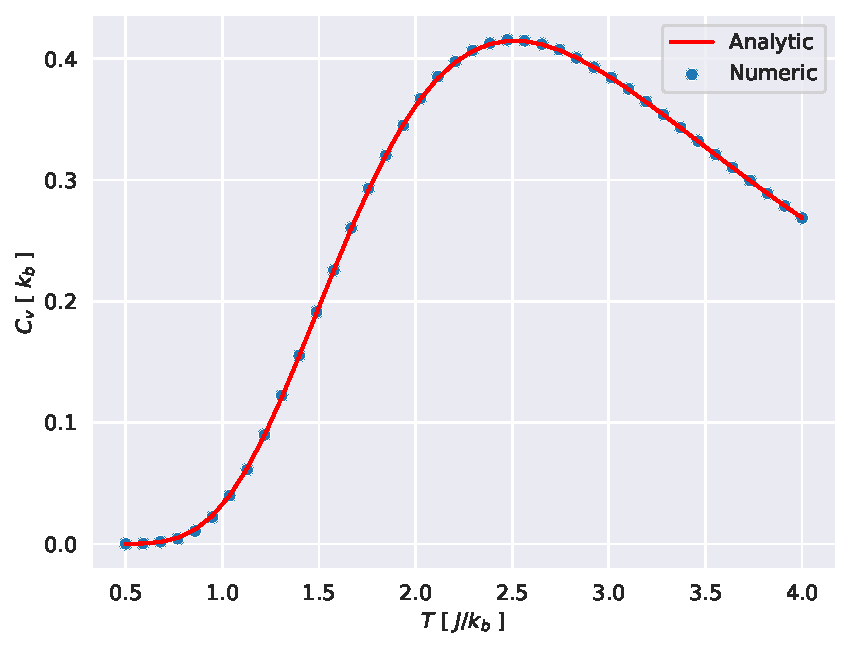
\includegraphics[width=.5\textwidth]{../figures/numeric_analytic_c_v_T.pdf}
    \caption{Comparison of the red analytic and blue numeric results in a $2\times2$ lattice case. Here one sees the expectation value for the heat capacity $C_V$ (normalized to number of spins) plotted against different temperatures $T$. Numerical results shown are for $10^6$ MC cycles.}
    \label{fig:numeric_analytic_c_v_T}
\end{figure}

\begin{figure}[H]
    \centering
    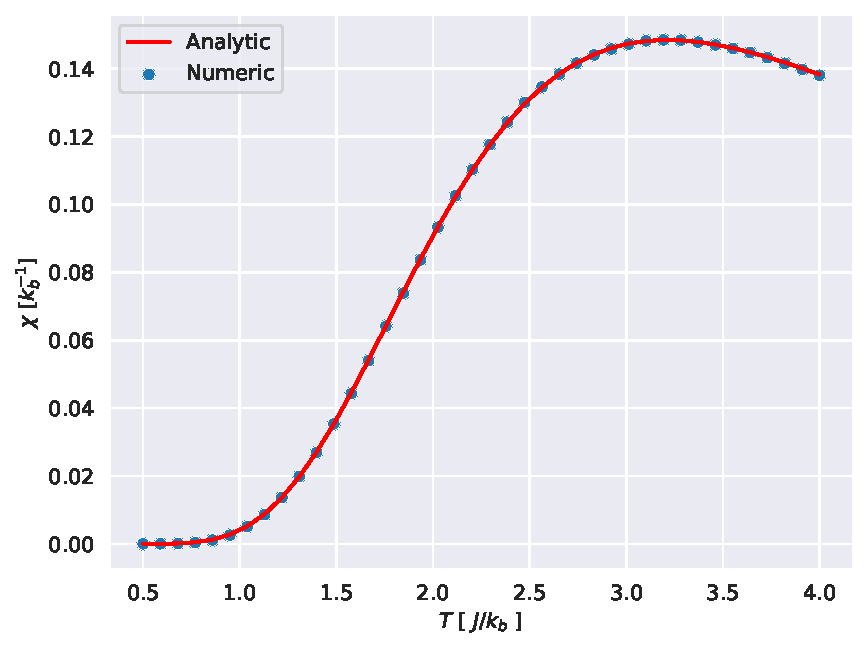
\includegraphics[width=.5\textwidth]{../figures/numeric_analytic_X_T.pdf}
    \caption{Comparison of the red analytic and blue numeric results in a $2\times2$ lattice case. Here one sees the expectation value for the susceptibility $\chi$ (normalized to number of spins) plotted against different temperatures $T$. Numerical results shown are for $10^6$ MC cycles.}
    \label{fig:numeric_analytic_X_T}
\end{figure}

Figures \ref{fig:numeric_analytic_e_T}, \ref{fig:numeric_analytic_m_T}, \ref{fig:numeric_analytic_c_v_T} and \ref{fig:numeric_analytic_X_T} show excellent agreement between numerical MCMC results and analytical results for the whole range of temperatures shown.

% diff of all four vlaues plot
\begin{figure}[H]
    \centering
    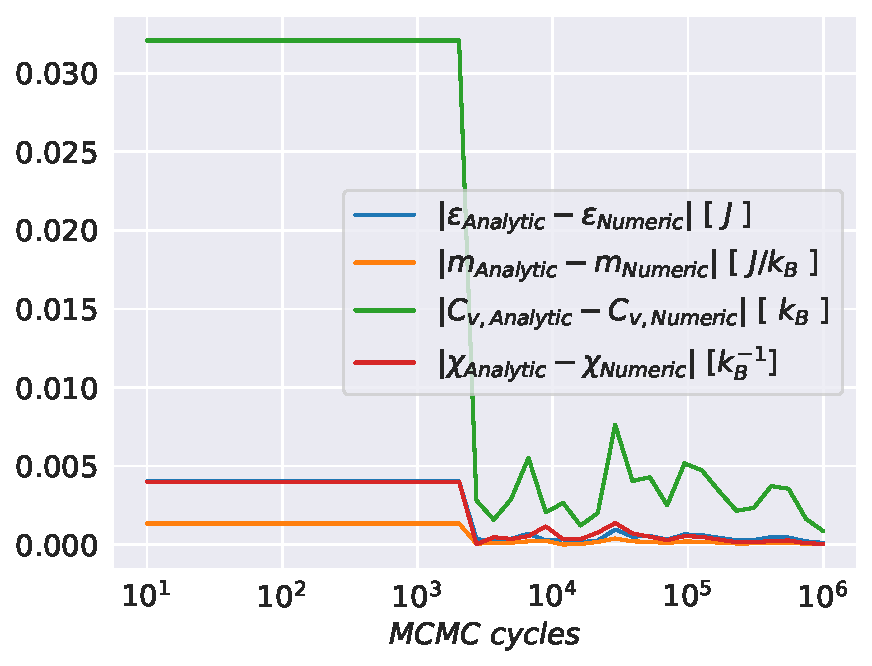
\includegraphics[width=.5\textwidth]{../figures/numeric_analytic.pdf}
    \caption{The blue, yellow, green and red line show the change of the difference between numerical and analytical results as a function of MCMC cycles for $\langle \epsilon \rangle$, $\langle |m| \rangle$, $C_V$ and $\chi$ respectively. In this case $L=2$ and the results are presented on a log scale.}
    \label{fig:numeric_analytic}
\end{figure}
In figure \ref{fig:numeric_analytic} one can see how the difference between numerical and analytical results decreases for increasing MCMC cycles. After about $10^{5}$ cycles the numerical results stabilize and are in good agreement with the analytical result for a $2 \times 2$ lattice. Further computations will be run for $10^6$ cycles to ensure precision since enough computational power is available.

This allows us to move on to more complex computations of larger lattice sizes. The next figures show results to study the \textbf{burn-in} time for our MCMC method for a $20 \times 20$ lattice. Results are shown for both a lattice with random spins and an ordered lattice with all spins starting in an up $(\uparrow)$ state.

% study burn in time for L=20
\begin{figure}[H]
    \centering
    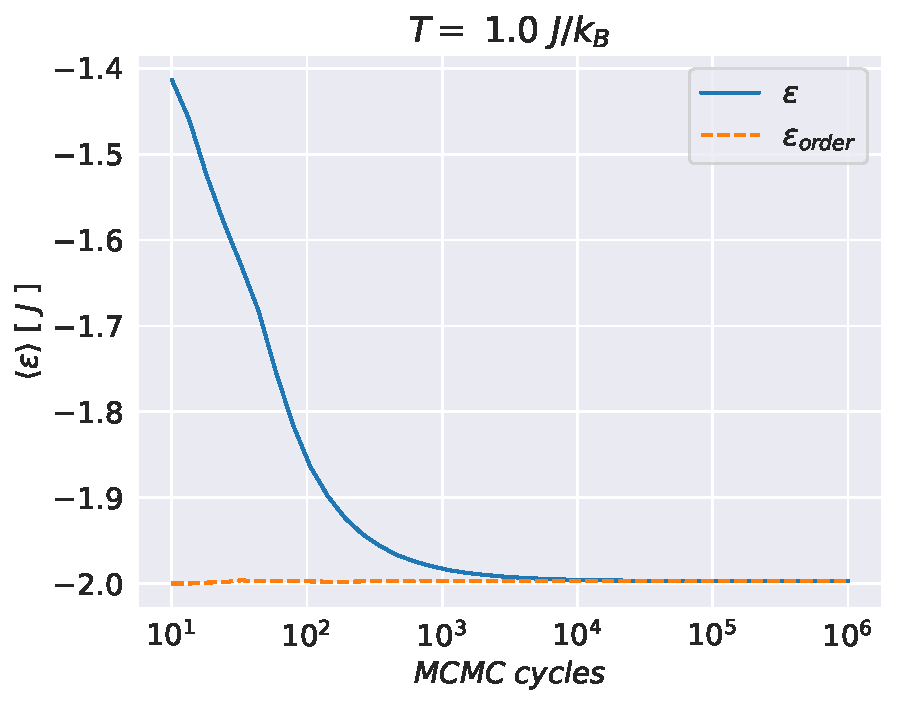
\includegraphics[width=.5\textwidth]{../figures/numeric_L_20_T_1_e.pdf}
    \caption{Numerical approximation values for $\langle \epsilon \rangle$ against number of MCMC cycles for $T=1.0 J/k_B$. The blue line shows the evolution from a random spin configuration whereas the orange line is for the case of an ordered spin configuration. Here $L=20$ and the results are presented on a log scale.}
    \label{fig:numeric_L_20_T_1_e}
\end{figure}

\begin{figure}[H]
    \centering
    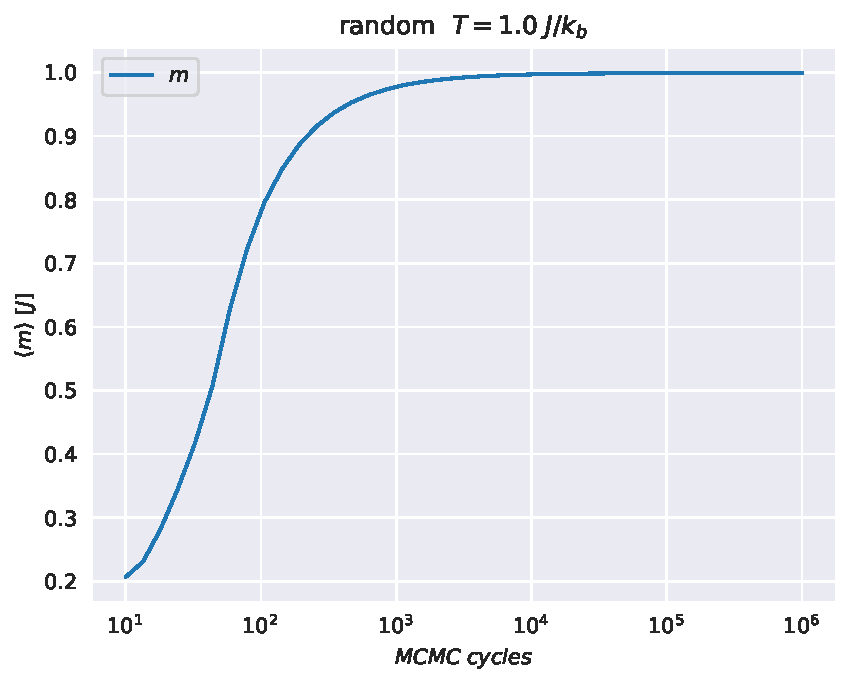
\includegraphics[width=.5\textwidth]{../figures/numeric_L_20_T_1_m.pdf}
    \caption{Numerical approximation values for $\langle |m| \rangle$ against number of MCMC cycles for $T=1.0 J/k_B$. The blue line shows the evolution from a random spin configuration whereas the orange line is for the case of an ordered spin configuration. Here $L=20$ and the results are presented on a log scale.}
    \label{fig:numeric_L_20_T_1_m}
\end{figure}
Figure \ref{fig:numeric_L_20_T_1_e} and \ref{fig:numeric_L_20_T_1_m} show that the MCMC method has a burn-in time of about $10^4$ cycles for $T=1.0J/k_B$ in an unordered spin case. Starting with ordered spins there is no burn-in time at all.

\begin{figure}[H]
    \centering
    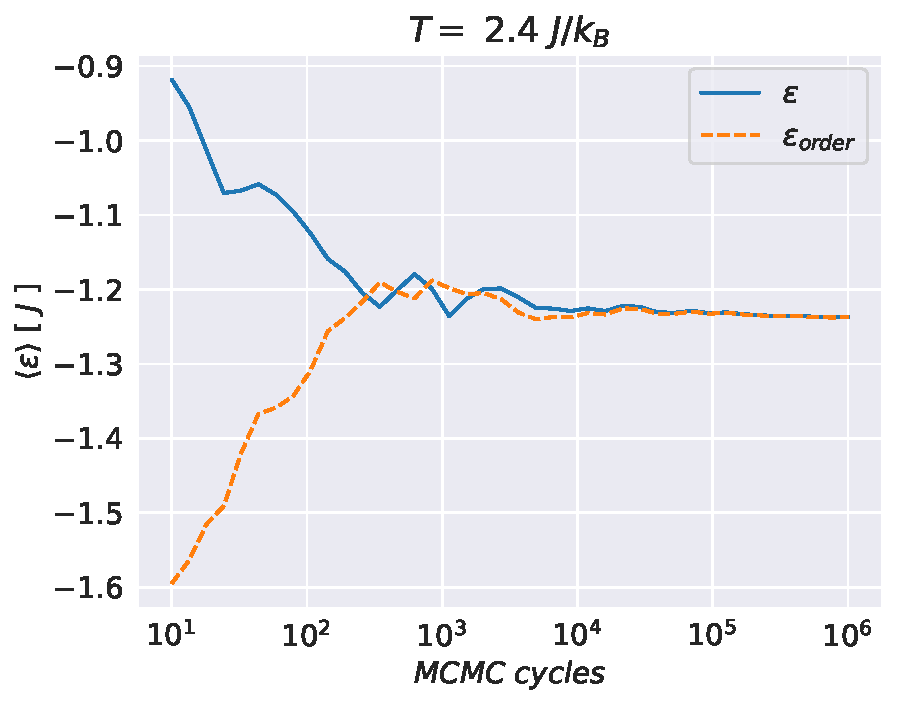
\includegraphics[width=.5\textwidth]{../figures/numeric_L_20_T_2_4_e.pdf}
    \caption{Numerical approximation values for $\langle \epsilon \rangle$ against number of MCMC cycles for $T=2.4 J/k_B$. The blue line shows the evolution from a random spin configuration whereas the orange line is for the case of an ordered spin configuration. Here $L=20$ and the results are presented on a log scale.}
    \label{fig:numeric_L_20_T_2_4_e}
\end{figure}

\begin{figure}[H]
    \centering
    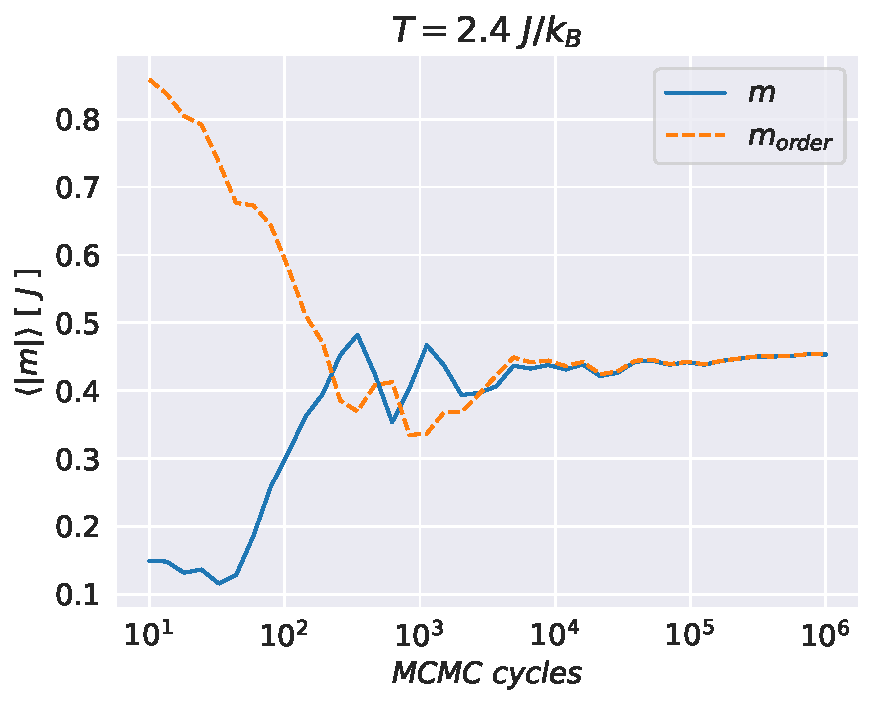
\includegraphics[width=.5\textwidth]{../figures/numeric_L_20_T_2_4_m.pdf}
    \caption{Numerical approximation values for $\langle |m| \rangle$ against number of MCMC cycles for $T=2.4 J/k_B$. The blue line shows the evolution from a random spin configuration whereas the orange line is for the case of an ordered spin configuration. Here $L=20$ and the results are presented on a log scale.}
    \label{fig:numeric_L_20_T_2_4_m}
\end{figure}
For $T=1.0J/k_B$ we see that the values for $\langle \epsilon \rangle$ in figure \ref{fig:numeric_L_20_T_2_4_e} and equally for $\langle |m| \rangle$ in figure \ref{fig:numeric_L_20_T_2_4_m} are fairly stable around $10^4$. The full burn-in time looks to be around $10^5$ cycles for both ordered and unordered spins.

Moving beyond expectation values we approximate the probability function $p_{\epsilon}(\epsilon ; T)$ using MCMC samples. This is done for both $T=1.0J/k_B$ and $T=2.4J/k_B$.
%histograms
\begin{figure}[H]
    \centering
    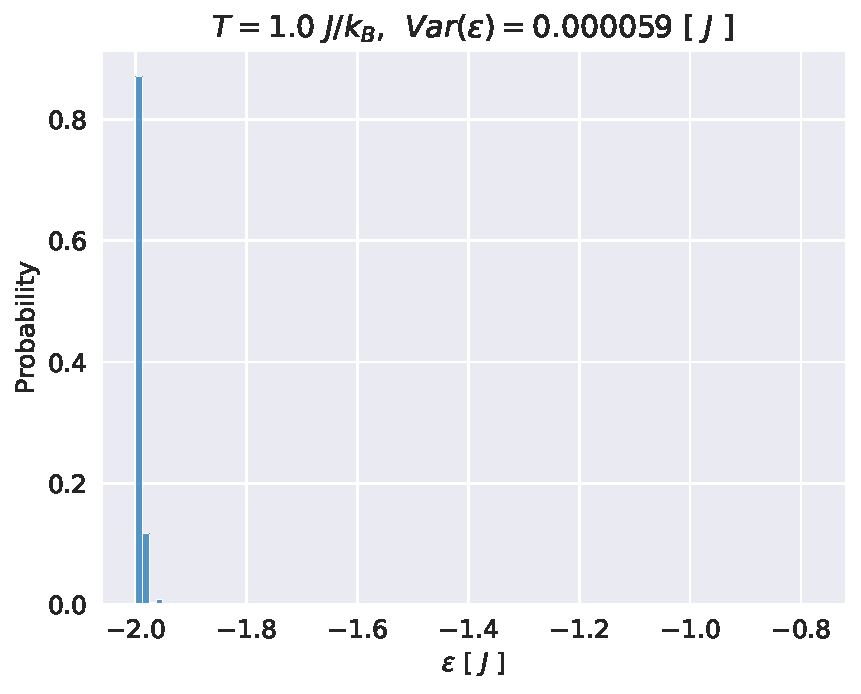
\includegraphics[width=.5\textwidth]{../figures/histogram_T_1_m.pdf}
    \caption{Approximation of the probability function $p_{\epsilon}(\epsilon ; T)$ for $L=20$ and $T=1.0 J/k_B$.}
    \label{fig:histogram_T_1_m}
\end{figure}

\begin{figure}[H]
    \centering
    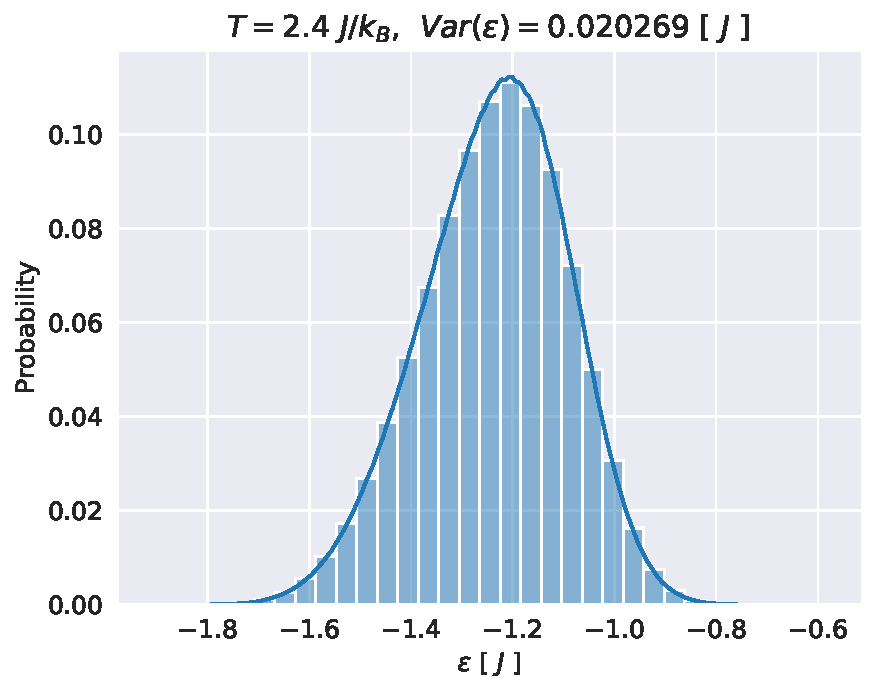
\includegraphics[width=.5\textwidth]{../figures/histogram_T_2_4_m.pdf}
    \caption{Approximation of the probability function $p_{\epsilon}(\epsilon ; T)$ for $L=20$ and $T=2.4 J/k_B$. The blue line shows the kernel distribution estimation of the histogram.}
    \label{fig:histogram_T_2_4_m}
\end{figure}
Comparing figure \ref{fig:histogram_T_1_m} for $T=1.0 J/k_B$ and figure \ref{fig:histogram_T_2_4_m} for $T=2.4 J/k_B$ the most noticeable result is the difference in variance. For $T=1.0 J/k_B$ an $\epsilon \approx -2$ is by far the most likely, whilst possible $\epsilon$ values for $T=2.4 J/k_B$ cover a larger range of approximately $[-1.7,-0.9]J/k_B$.

\begin{figure}[H]
    \centering
    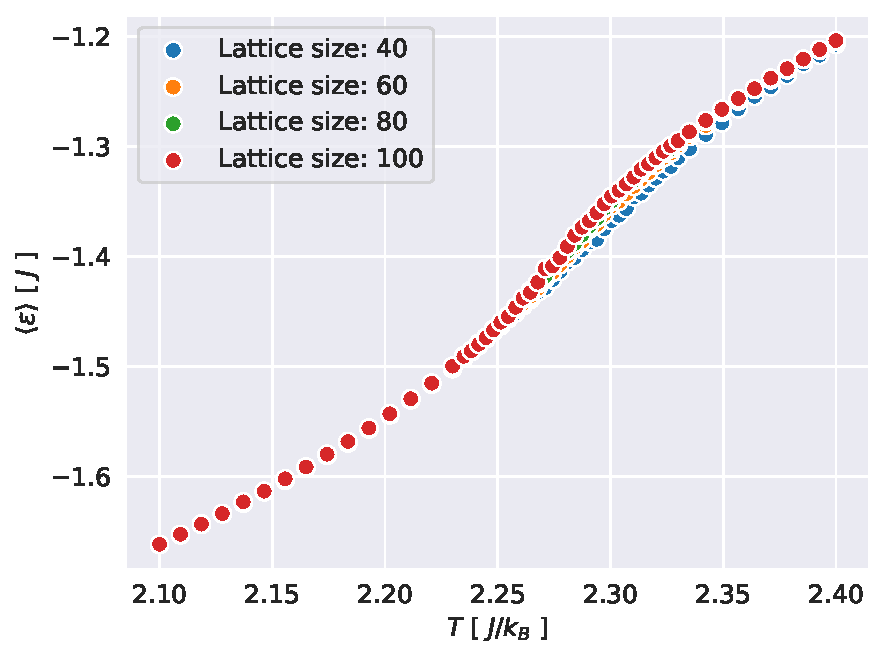
\includegraphics[width=.5\textwidth]{../figures/L_size_e_T.pdf}
    \caption{$\langle \epsilon \rangle$ is shown as a function of temperature $T$ for lattice size $L= 40, 60,80,100$.}
    \label{fig:L_size_e_T}
\end{figure}

\begin{figure}[H]
    \centering
    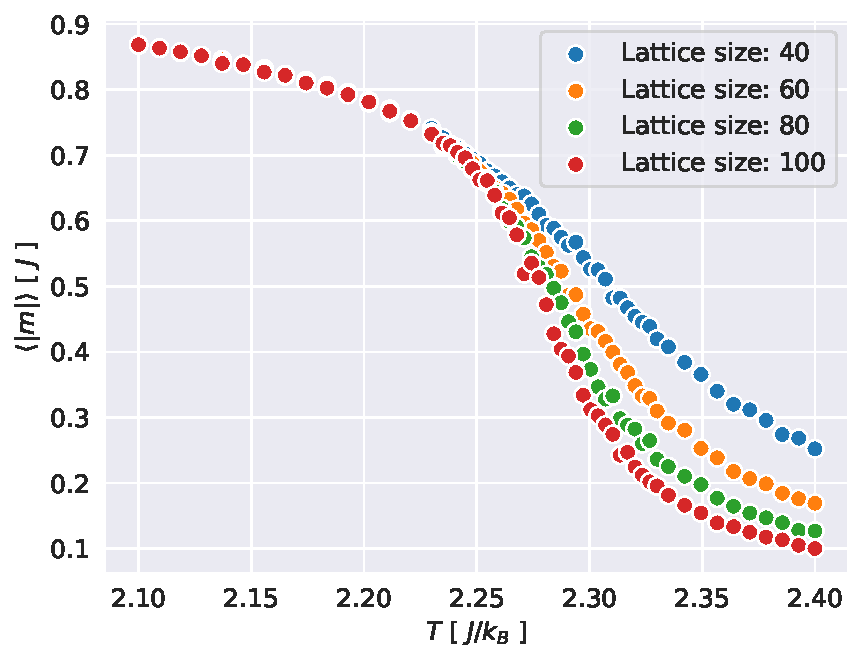
\includegraphics[width=.5\textwidth]{../figures/L_size_m_T.pdf}
    \caption{$\langle |m| \rangle$ is shown as a function of temperature $T$ for lattice size $L= 40, 60,80,100$.}
    \label{fig:L_size_m_T}
\end{figure}
Figure \ref{fig:L_size_e_T} shows small variations in mean energy for increasing lattice size $L$. Looking closely in at $T \in [2.22,2.4]J/k_B$ one can see that $\langle \epsilon \rangle$ increases slightly with increasing $L$. In figure \ref{fig:L_size_m_T} the mean magnetization changes more noticeably for different $L$. $\langle |m| \rangle$ tends toward zero for increasing $T$ and noticeably the graphs slope steepens around $T \in [2.25,2.30]J/k_B$ for increasing lattice sizes.

\begin{figure}[H]
    \centering
    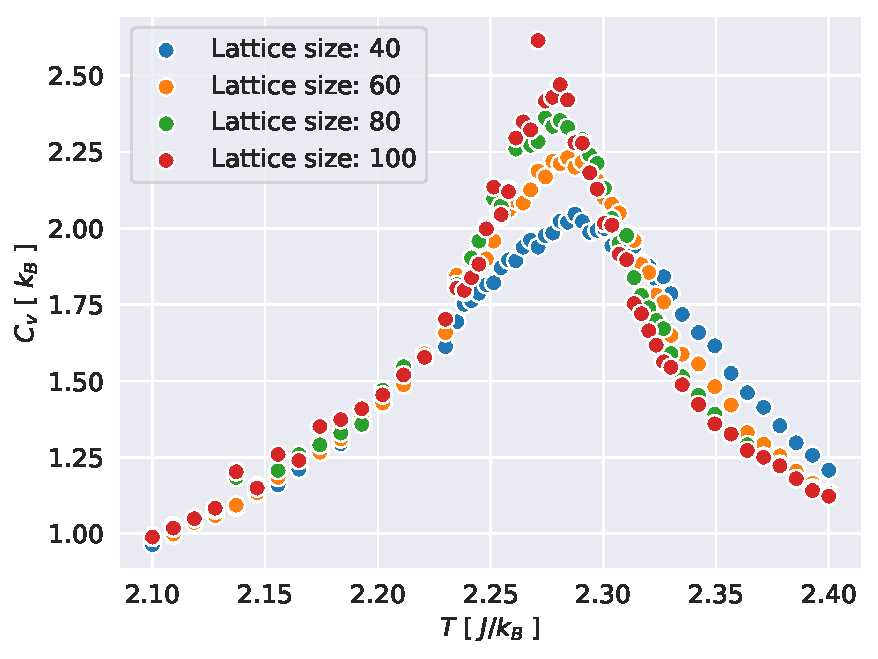
\includegraphics[width=.5\textwidth]{../figures/L_size_c_v_T.pdf}
    \caption{$C_V$ is shown as a function of temperature $T$ for lattice size $L= 40, 60,80,100$.}
    \label{fig:L_size_c_v_T}
\end{figure}

\begin{figure}[H]
    \centering
    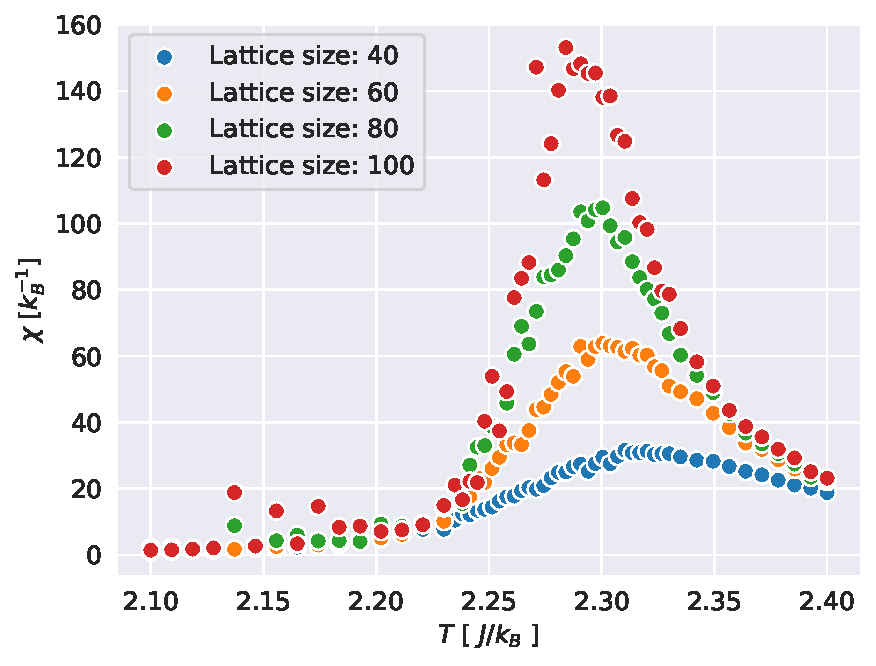
\includegraphics[width=.5\textwidth]{../figures/L_size_X_T.pdf}
    \caption{$\chi$ is shown as a function of temperature $T$ for lattice size $L= 40, 60,80,100$.}
    \label{fig:L_size_X_T}
\end{figure}
The specific heat capacity in figure \ref{fig:L_size_c_v_T} increases for $T \in [2.25,2.30]J/k_B$ with increasing lattice size. In figure \ref{fig:L_size_X_T} the susceptibility shows similar behavior to the heat capacity with an increase of $\chi$ for larger lattice sizes in the region of  $T \in [2.25,2.35]J/k_B$. In both cases the peak value for a $40 \times 40$ lattice is around $T=2.30J/k_B$. As the lattice size increases, the peak $C_V$ and $\chi$ trend towards a lower temperature. For all four figures above a smaller $\Delta T$ has been chosen for $T > 2.235J/k_B$, specifically for  $T \in [2.235,2.33]J/k_B$ we have $\Delta T = 0.003J/k_B$.

\begin{table}
    \centering
    \caption{Critical temperature as a function of lattice size computed using both $\chi$ and $C_v$.}
    \label{tab:critical_T}
    \begin{tabular}{|c|c|c|c|c|}
        \hline
        Lattice sizes                & 40    & 60    & 80    & 100   \\
        \hline
        $T_C$ using $C_V$ [$J/k_B$]  & 2.287 & 2.284 & 2.274 & 2.271 \\
        \hline
        $T_C$ using $\chi$ [$J/k_B$] & 2.310 & 2.300 & 2.301 & 2.284 \\
        \hline
    \end{tabular}
\end{table}
\begin{figure}[H]
    \centering
    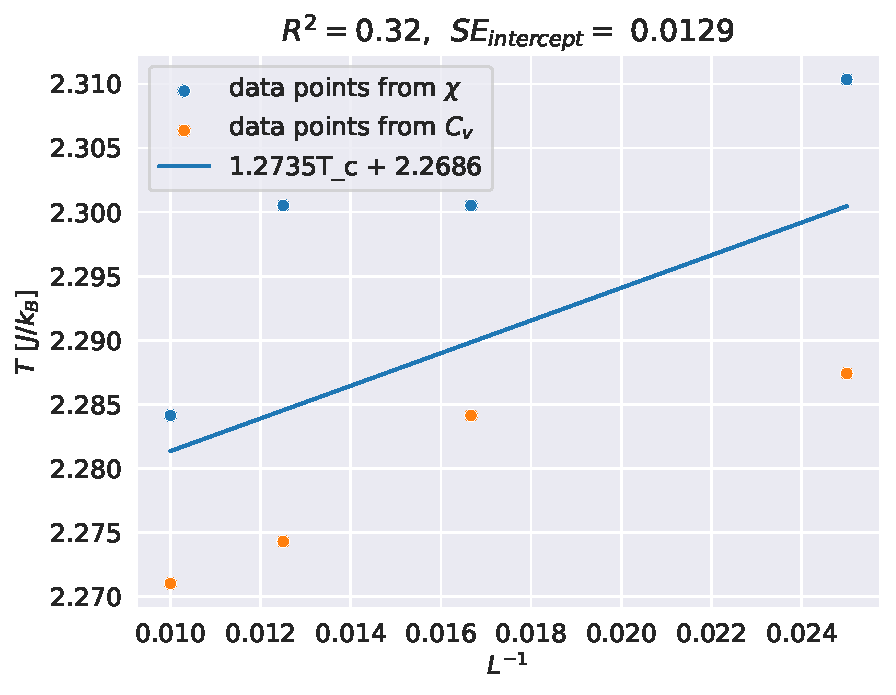
\includegraphics[width=.5\textwidth]{../figures/linregress.pdf}
    \caption{The blue line shows linear regression using critical temperature points $T_c$ from $\chi$ and $C_V$ for different lattice sizes $L$. Here temperature $T$ is plotted against $L^{-1}$.}
    \label{fig:linregress}
\end{figure}
Taking the temperature values at the peak values of the specific heat capacity $C_V$ and the susceptibility $\chi$ show in table \ref{tab:critical_T} and performing linear regression results in the blue line in figure \ref{fig:linregress}. We have the function
\begin{equation}
    T_c(L) = 1.2735 L^{-1} + 2.2686.
\end{equation}
This gives us $a=1.2735$ and letting $L=\infty$ we have
\begin{equation}
    T_c(L=\infty) = 2.2686 J/k_B
\end{equation}
with a standard error of $0.0129 J/k_B$.

\begin{table}[H]
    \centering
    \caption{Time used for different number of threads in parallelization at temperature level. A quad-core, 8 thread CPU has been used for the ising model initialized with a $5\times5$ lattice with randomized initial spins and temperature $T= 1$ $J/k_B$}
    \label{tab:timing}
    \begin{tabular}{|c|c|c|c|}
        \hline
        Number of threads & 1     & 4    & 8    \\
        \hline
        Time used (s)     & 29.12 & 8.42 & 7.32 \\
        \hline
        speed-up factor   & 1     & 3.45 & 3.92 \\
        \hline
    \end{tabular}
\end{table}
In table \ref{tab:timing} we see that parallelizing our code can reduce computation time a factor of 0.25 using 8 threads for an 8 thread CPU. We also see that a 4 thread parallelization performs well with a speed-up factor of 3.45.
% ===========================================
\section{Discussion}\label{sec:discussion}
% numerical analytucal comparisson and reasonable agreement for L=2
We start by testing our numerical Ising model simulation against analytical results for a $2 \times 2$ lattice to ensure its functionality. The results in figures \ref{fig:numeric_analytic_e_T}, \ref{fig:numeric_analytic_m_T}, \ref{fig:numeric_analytic_c_v_T} and \ref{fig:numeric_analytic_X_T} show excellent agreement over $T \in [0.5, 4.0]J/k_B$ for $10^6$ MCMC cycles. This shows the MCMC method is a suitable choice for this complex Ising model problem. Taking a closer look at the amount of cycles necessary for good agreement in figure \ref{fig:numeric_analytic} confirms that at least $10^5$ MCMC cycles are necessary for a precise numerical approximation. All further simulations are therefore run for $10^6$ cycles. $10^7$ would definitely give even better results, but also come at a large run time cost.

% burn-in time for L=20 and approximating probability distribution
Studying the burn-in time (i.e. the time it takes for the algorithm to stabilize on the correct values) for a $20 \times 20$ lattice for $T=1.0 J/k_B$ in figure \ref{fig:numeric_L_20_T_1_e} and \ref{fig:numeric_L_20_T_1_m} we see that the only noticeable burn-in time is for the unordered spin case. For $\epsilon$ in figure \ref{fig:numeric_L_20_T_1_e} this is between $10^3$ and $10^4$ cycles. This explains the small variance in figure \ref{fig:histogram_T_1_m} which is run for $10^6$ cycles, thus gathering an enormous amount of samples after the burn-in time. The ordered case of all spins being up already matches the expected energy, thus not having a burn-in time.

Figure \ref{fig:numeric_L_20_T_2_4_e} and \ref{fig:numeric_L_20_T_2_4_m} for $T=2.4 J/k_B$ on the other hand, show a slightly longer burn-in time closer to $10^5$ cycles. In this case the ordered spin configuration does not instantly match the expected values resulting in more similar behavior for the ordered and unordered burn-in time. The burn-in time for $\langle \epsilon \rangle$ at $T=2.4J/k_B$ in figure \ref{fig:numeric_L_20_T_2_4_e} is longer than in the $T=1.0 J/k_B$ case explaining the larger variance in figure \ref{fig:histogram_T_2_4_m} compared to figure \ref{fig:histogram_T_1_m}. One can also see some oscillatory behavior matching the almost even distribution to both sides of $-1.2 J$ in figure \ref{fig:histogram_T_2_4_m}.

It could be argued that more precise results can be generated if one chooses not to use samples from the burn-in time. This is because a very unlikely initial state can affect the final distribution since a large amount of the samples generated are actually highly unlikely. A solution to this, and what we have chosen to do, is to run as many cycles as is computationally reasonable when considering runtimes. Based on the burn-in time results, running $10^6$ cycles seems enough to out way any highly unlikely initial spin configuration. At least in the $L=20$ case. Whether this is actually true for larger lattice sizes as well would require further testing.

%approximation of L=\infty
Having developed a certain understanding and confidence in our model we now start looking for indications of phase transition. One can see that the mean magnetization drops off more abruptly after $T=2.25 J/k_B$ in figure \ref{fig:L_size_m_T}. This matches the expected phase transition for the Ising model which is a loss of magnetization after a certain critical temperature $T_c$. Seeing how the graphs slope steepens for increasing $L$ we would expect it to be infinitely steep in an infinite lattice case at $T_c$. Studying the region $T \in [2.235,2.33]J/k_B$ in figure \ref{fig:L_size_c_v_T} and \ref{fig:L_size_X_T} we observe definite peak values for $C_V$ and $\chi$. This abrupt change from the change of the external temperature parameter further indicates a phase transition happening in this region of $T$. The critical temperature at which $C_V$ and $\chi$ peak for different lattice sizes is shown in table \ref{tab:critical_T}. The critical temperature at which the phase transition happens for an infinite lattice is then found in figure \ref{fig:linregress} using linear regression of the $T_c$ for different lattice sizes. Since the data set is fairly small we have chosen to use all eight data points. The resulting critical temperature approximation is
\begin{equation}
    T_c(L=\infty) = 2.2686 J/k_B.
\end{equation}
This is an excellent approximation of Onsager's analytical result of
\begin{equation}
    T_{c \text{ analytic}}(L=\infty) \approx 2.269 J/k_B
\end{equation}
confirming the Markov Chain Monte Carlo method's applicability to complex problem-solving. To improve the approximation one could use an even smaller $\Delta T$ and more lattice sizes. This would result in a more precise set of data points for the linear regression.

% optimization
Considering code optimization, we have chosen to parallelize the section of the code lopping over different temperatures and different numbers of cycles. This gives us time savings when we are plotting against these two variables, but not when running a single MCMC run. Another way of parallelizing the code would therefore be at the level of the MCMC ``walkers'' using several threads to execute multiple individual MCMC runs to finally combine the results.

% Timing

From our timing test using parallelization at temperature level we saw a great reduction in computation time when using more threads with a speed-up factor of 3.92 going from utilizing 1 to 8 threads. For an 8 thread CPU we would expect the speed-up factor being closer to 8, which shows that the physical core count of the processor influences the speed-up factor. In our case of a quad-core CPU we saw that even 4 threaded parallelization got close to the 8 thread performance. In total this means that the expected speed-up factor using all of a processor's threads would be closer to its physical core and not thread count. On the other hand, we do not know how parallelization at the level of the Markov Chain Monte Carlo method would influence the speed-up time. Such a parallelization may see better performance than our time level parallelization overall as well as better scaling when using more threads. This would require further investigation.


% ===========================================
\section{Conclusion}\label{sec:conclusion}
We have found the Markov Chain Monte Carlo method to give good approximations of mean energy, magnetization, heat capacity and susceptibility of the Ising model for different temperatures. The chosen $10^6$ MCMC cycles offers a good compromise between precision and computational cost. Studying the Ising model parameters' behavior over different temperatures such as in figure \ref{fig:L_size_c_v_T} shows indications of a phase tradition at a certain critical temperature $T_c$. Using eight data points of $T_c$ for four different lattice sizes we perform a linear regression allowing us to approximate the critical temperature for an infinite lattice. This results in $ T_c(L=\infty) = 2.2686 J/k_B$ with a standard error of $0.0129 J/k_B$. This is an impressive approximation of Onsager's analytical result of  $T_{c \text{ analytic}}(L=\infty) \approx 2.269 J/k_B$.
MORE ABOUT LOOSE ENDS AND FURTHER RESAERCH.


\onecolumngrid

%\bibliographystyle{apalike}
\bibliography{report4}

\newpage
\appendix
\raggedbottom

\section{Analytical solutions for a 2$\cross$2 lattice}\label{appendix:analytic}
For the case of a 2$\cross$2 lattice with $L=2$ and $N=4$ we have sixteen possible spin configurations show in table \ref{tab:analytic}. These values will be used for the analytic solutions. The specific partition function becomes
\begin{align*}
    Z & =  \sum_{\text{all possible \textbf{s}}} e^{- \beta E(\textbf{s})}
    = 2e^{- \beta (-8J)} + 2e^{- \beta 8J} + 12e^0
    = 2 e^{\beta 8J} + 2 e^{- \beta 8J} + 12
    = 4 (\cosh(8 \beta J) + 3).
\end{align*}
Additionally, we will calculate a few expectation values for which the general formula is given as
\begin{align*}
    \langle A \rangle = \sum_s A_s p(s).
\end{align*}
This is a sum over all spin states $s_i$. Here $p(s)$ is a chosen probability distribution, in our this case the Boltzmann distribution in eq. \ref{eq:prob_dist}. The fist and second of the following analytical derivations will use the hyperbolic function definition $\sinh(x) = \frac{e^x - e^{-x}}{2}$ and $\cosh(x) = \frac{e^x + e^{-x}}{2}$ respectively. For the energy we have
\begin{align*}
    \langle E \rangle          & =  \sum_s E(\textbf{s})  p(\textbf{s};T)
    = \frac{1}{Z} \sum_s E(\textbf{s})  e^{-\beta E(\textbf{s})}
    = \frac{1}{Z} \left( 2 \cdot (-8J)e^{\beta8J} + 2 \cdot 8J e^{-\beta 8J}\right)              \\
                               & = \frac{1}{Z} \left( -16 e^{\beta8J} + 16 e^{-\beta 8J}\right)
    = \frac{16J}{Z} \left( e^{-\beta 8J} - e^{\beta 8J} \right)
    = - \frac{32 J \sinh(8J \beta )}{Z},
    \\
    \\
    \langle E^2 \rangle        & =  \sum_s E(\textbf{s})^2  p(\textbf{s};T)
    = \frac{1}{Z} \sum_s E(\textbf{s})^2  e^{-\beta E(\textbf{s})}
    = \frac{1}{Z} \left( 2 \cdot (-8J)^2e^{\beta8J} + 2 \cdot (8J)^2 e^{-\beta 8J}\right)        \\
                               & = \frac{128 J^2}{Z} \left( e^{-\beta 8J} + e^{\beta 8J} \right)
    = \frac{256 J^2 \cosh(8J \beta)}{Z},
    \\
    \\
    \langle \epsilon \rangle   & =  \sum_s \epsilon_s  p(\textbf{s};T)
    =  \sum_s \frac{E(\textbf{s})}{N}  p(\textbf{s};T)
    =  \frac{1}{N} \sum_s E(\textbf{s})  p(\textbf{s};T)
    =  \frac{\langle E \rangle }{4}
    %= \frac{4J}{Z} \left( e^{-\beta 8J} - e^{\beta 8J} \right)
    = - \frac{8J \sinh(8J \beta)}{Z},
    \\
    \\
    \langle \epsilon^2 \rangle & =  \sum_s \epsilon_s^2  p(\textbf{s};T)
    =  \sum_s \left(\frac{E(\textbf{s})}{N}\right)^2  p(\textbf{s};T)
    =  \frac{1}{N^2} \sum_s E(\textbf{s})^2  p(\textbf{s};T)
    =  \frac{\langle E^2 \rangle }{16}
    %= \frac{8 J^2}{Z} \left( e^{-\beta 8J} + e^{\beta 8J} \right)
    = \frac{16 J^2 \cosh(8J \beta)}{Z}.
\end{align*}
Then for the magnetization we have
\begin{align*}
    \langle |M| \rangle & =  \sum_s |M(\textbf{s})|  p(\textbf{s};T)
    = \frac{1}{Z} \sum_s |M(\textbf{s})| e^{-\beta E(\textbf{s})}
    = \frac{1}{Z} \left( |-4|e^{\beta8J} + 4 |-2| e^0 + 4|2|e^0 + |4|e^{\beta 8J}\right)            \\
                        & = \frac{1}{Z} \left( 4e^{\beta8J} + 8 + 8 + 4e^{\beta 8J}\right)
    = \frac{8}{Z} \left( e^{\beta 8J} + 2 \right),
    \\
    \\
    \langle M^2 \rangle & = \sum_s M(\textbf{s})^2  p(\textbf{s};T)
    = \frac{1}{Z} \sum_s M(\textbf{s})^2 e^{-\beta E(\textbf{s})}
    = \frac{1}{Z} \left( (-4)^2 e^{\beta8J} + 4 (-2)^2 e^0 + 4(2)^2 e^0 + (4)^2 e^{\beta 8J}\right) \\
                        & = \frac{1}{Z} \left( 16 e^{\beta8J} + 16 + 16 + 16 e^{\beta 8J}\right)
    = \frac{32}{Z} \left( e^{\beta 8J} + 1 \right),
    \\
    \\
    \langle |m| \rangle & = \sum_s |m(\textbf{s})|  p(\textbf{s};T)
    = \frac{1}{Z} \sum_s \bigg| \frac{M(\textbf{s})}{N} \bigg| e^{-\beta E(\textbf{s})}
    = \frac{\langle|M| \rangle}{4}
    = \frac{2}{Z} \left( e^{\beta 8J} + 2 \right),
    \\
    \\
    \langle m^2 \rangle & = \sum_s m(\textbf{s})^2  p(\textbf{s};T)
    = \frac{1}{Z} \sum_s \left( \frac{M(\textbf{s})}{N} \right)^2 e^{-\beta E(\textbf{s})}
    = \frac{ \langle M^2 \rangle}{4^2}
    = \frac{ \langle M^2 \rangle}{16}
    = \frac{2}{Z} \left( e^{\beta 8J} + 1 \right).
\end{align*}

Finally, we find analytical expressions for the specific heat capacity
\begin{align*}
    C_V = \frac{1}{N} \frac{1}{k_B T^2} \left( \langle E^2 \rangle - \langle E \rangle^2 \right)
    = \frac{1}{4} \frac{1}{k_B T^2} \left( \frac{256 J^2 \cosh(8J \beta)}{Z} - \left( - \frac{32 J \sinh(8J \beta )}{Z} \right)^2 \right)
    ,
\end{align*}
and the susceptibility
\begin{align*}
    \chi = \frac{1}{N} \frac{1}{k_B T} \left( \langle M^2 \rangle - \langle |M| \rangle^2 \right)
    = \frac{1}{4} \frac{1}{k_B T} \left( \frac{32}{Z} \left( e^{\beta 8J} + 1 \right) - \left( \frac{8}{Z} \left( e^{\beta 8J} + 2 \right) \right)^2 \right).
\end{align*}


\section{Possible $\Delta E$ values}\label{appendix:delta_E}
Considering a 2D lattice of arbitrary size $(L>2)$ and remembering that we are working with periodic boundary conditions, we can show that there are only a few possible values of $\Delta E$. The calculation of $\Delta E$ between spin configurations will be limited to the flipping of a single spin. To find the possible energy differences we will look at a spin at a random position. This central spin will start in an up state(+1) and then be flipped (-1). We remind that $ E(\textbf{s}) = - J \sum^4_{\langle kl \rangle} s_k s_l$ and $ \Delta E = E_{\text{after}} - E_{\text{before}}$.
\begin{table}[H]
    %\centering
    \begin{tabular}{llll}
                   & $\uparrow$ &            \\
        $\uparrow$ & $\uparrow$ & $\uparrow$ \\
                   & $\uparrow$ &
    \end{tabular}
    has $E = -4J$, now flipping we have
    \begin{tabular}{llll}
                   & $\uparrow$   &            \\
        $\uparrow$ & $\downarrow$ & $\uparrow$ \\
                   & $\uparrow$   &
    \end{tabular}
    and $E = 4J$, resulting in $\Delta E = 8J$.
\end{table}
This can be show for the four remaining possible starting configurations as well.
\begin{table}[H]
    %\centering
    \begin{tabular}{llll}
                     & $\uparrow$ &            \\
        $\downarrow$ & $\uparrow$ & $\uparrow$ \\
                     & $\uparrow$ &
    \end{tabular}
    has $E = -2J$. Flipping we have
    \begin{tabular}{llll}
                     & $\uparrow$   &            \\
        $\downarrow$ & $\downarrow$ & $\uparrow$ \\
                     & $\uparrow$   &
    \end{tabular}
    and $E = 2J$, resulting in $\Delta E = 4J$.
\end{table}

\begin{table}[H]
    %\centering
    \begin{tabular}{llll}
                     & $\uparrow$   &            \\
        $\downarrow$ & $\uparrow$   & $\uparrow$ \\
                     & $\downarrow$ &
    \end{tabular}
    has $E = 0$. Flipping we have
    \begin{tabular}{llll}
                     & $\uparrow$   &            \\
        $\downarrow$ & $\downarrow$ & $\uparrow$ \\
                     & $\downarrow$ &
    \end{tabular}
    and $E = 0$, resulting in $\Delta E = 0$.
\end{table}

\begin{table}[H]
    %\centering
    \begin{tabular}{llll}
                     & $\uparrow$   &              \\
        $\downarrow$ & $\uparrow$   & $\downarrow$ \\
                     & $\downarrow$ &
    \end{tabular}
    has $E = 2J$. Flipping we have
    \begin{tabular}{llll}
                     & $\uparrow$   &              \\
        $\downarrow$ & $\downarrow$ & $\downarrow$ \\
                     & $\downarrow$ &
    \end{tabular}
    and $E = -2J$, resulting in $\Delta E = -4J$.
\end{table}

\begin{table}[H]
    %\centering
    \begin{tabular}{llll}
                     & $\downarrow$ &              \\
        $\downarrow$ & $\uparrow$   & $\downarrow$ \\
                     & $\downarrow$ &
    \end{tabular}
    has $E = 4J$. Flipping we have
    \begin{tabular}{llll}
                     & $\downarrow$ &              \\
        $\downarrow$ & $\downarrow$ & $\downarrow$ \\
                     & $\downarrow$ &
    \end{tabular}
    and $E = -4J$, resulting in $\Delta E = -8J$.
\end{table}
The five possible values of the energy difference are thus, $\Delta E = 8J, 4J, 0, -4J, -8J$.

\newpage
\section{Theoretical background for critical phenomena}\label{appendix:critical}
Power laws with so-called critical exponents describe how a physical system behaves when close to its critical point. For the Ising model this is close to its critical temperature. For temperatures $T$ close to $T_c$ the \textit{infinite} 2D Ising model's mean magnetization, heat capacity and susceptibility behave as follows:
\begin{align*}
    \langle |m| \rangle & \propto |T-T_c(L = \infty)|^\beta,     \\
    C_V                 & \propto |T-T_c(L = \infty)|^{-\alpha}, \\
    \chi                & \propto |T-T_c(L = \infty)|^{-\gamma}.
\end{align*}
Here $\beta = 1/8$, $\alpha = 0$ and $\gamma = 7/4$ are the critical exponents. We see that $C_V$ and $\chi$ diverge close to $T_c$. The \textit{correlation length}
\begin{equation}
    \xi \propto |T-T_c(L=\infty)|^{-\nu} \label{eq:xi}
\end{equation}
with $\nu=1$ also diverges near $T_c$. For our finite system $\xi = L$ is the largest correlation length. Replacing for $\xi$ in eq. \ref{eq:xi} then leads to the scaling equation
\begin{equation}
    T_c(L) -T_c(L=\infty) = aL^{-1}.
\end{equation}

\section{Metropolis algorithm flow chart}\label{appendix:metro}

\begin{figure}[H]
    \centering
    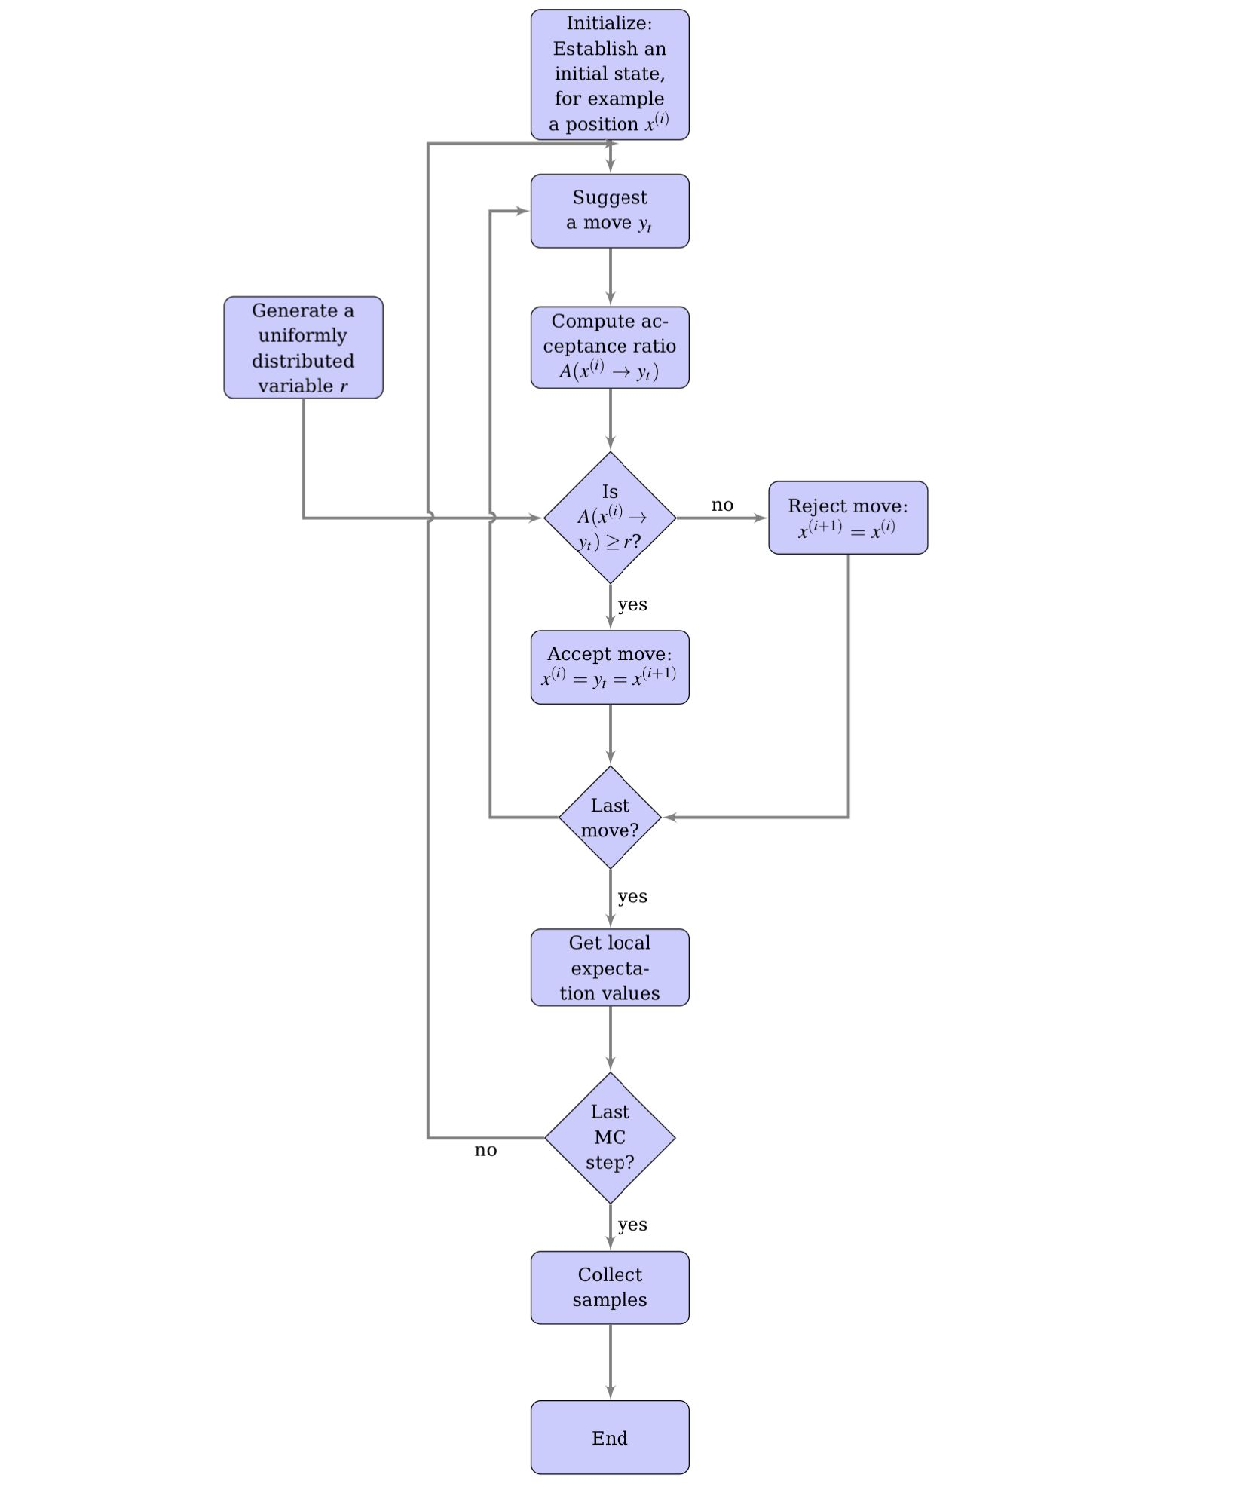
\includegraphics[width=1\textwidth]{../figures//metro_flow.pdf}
    \caption{Flowchart of the Metropolis algorithm taken from Computational Physics lecture notes \cite{compedium}.}
    \label{fig:metro_flow}
\end{figure}

\end{document}